Scan at NLO

\begin{figure}[hbt]
\centering
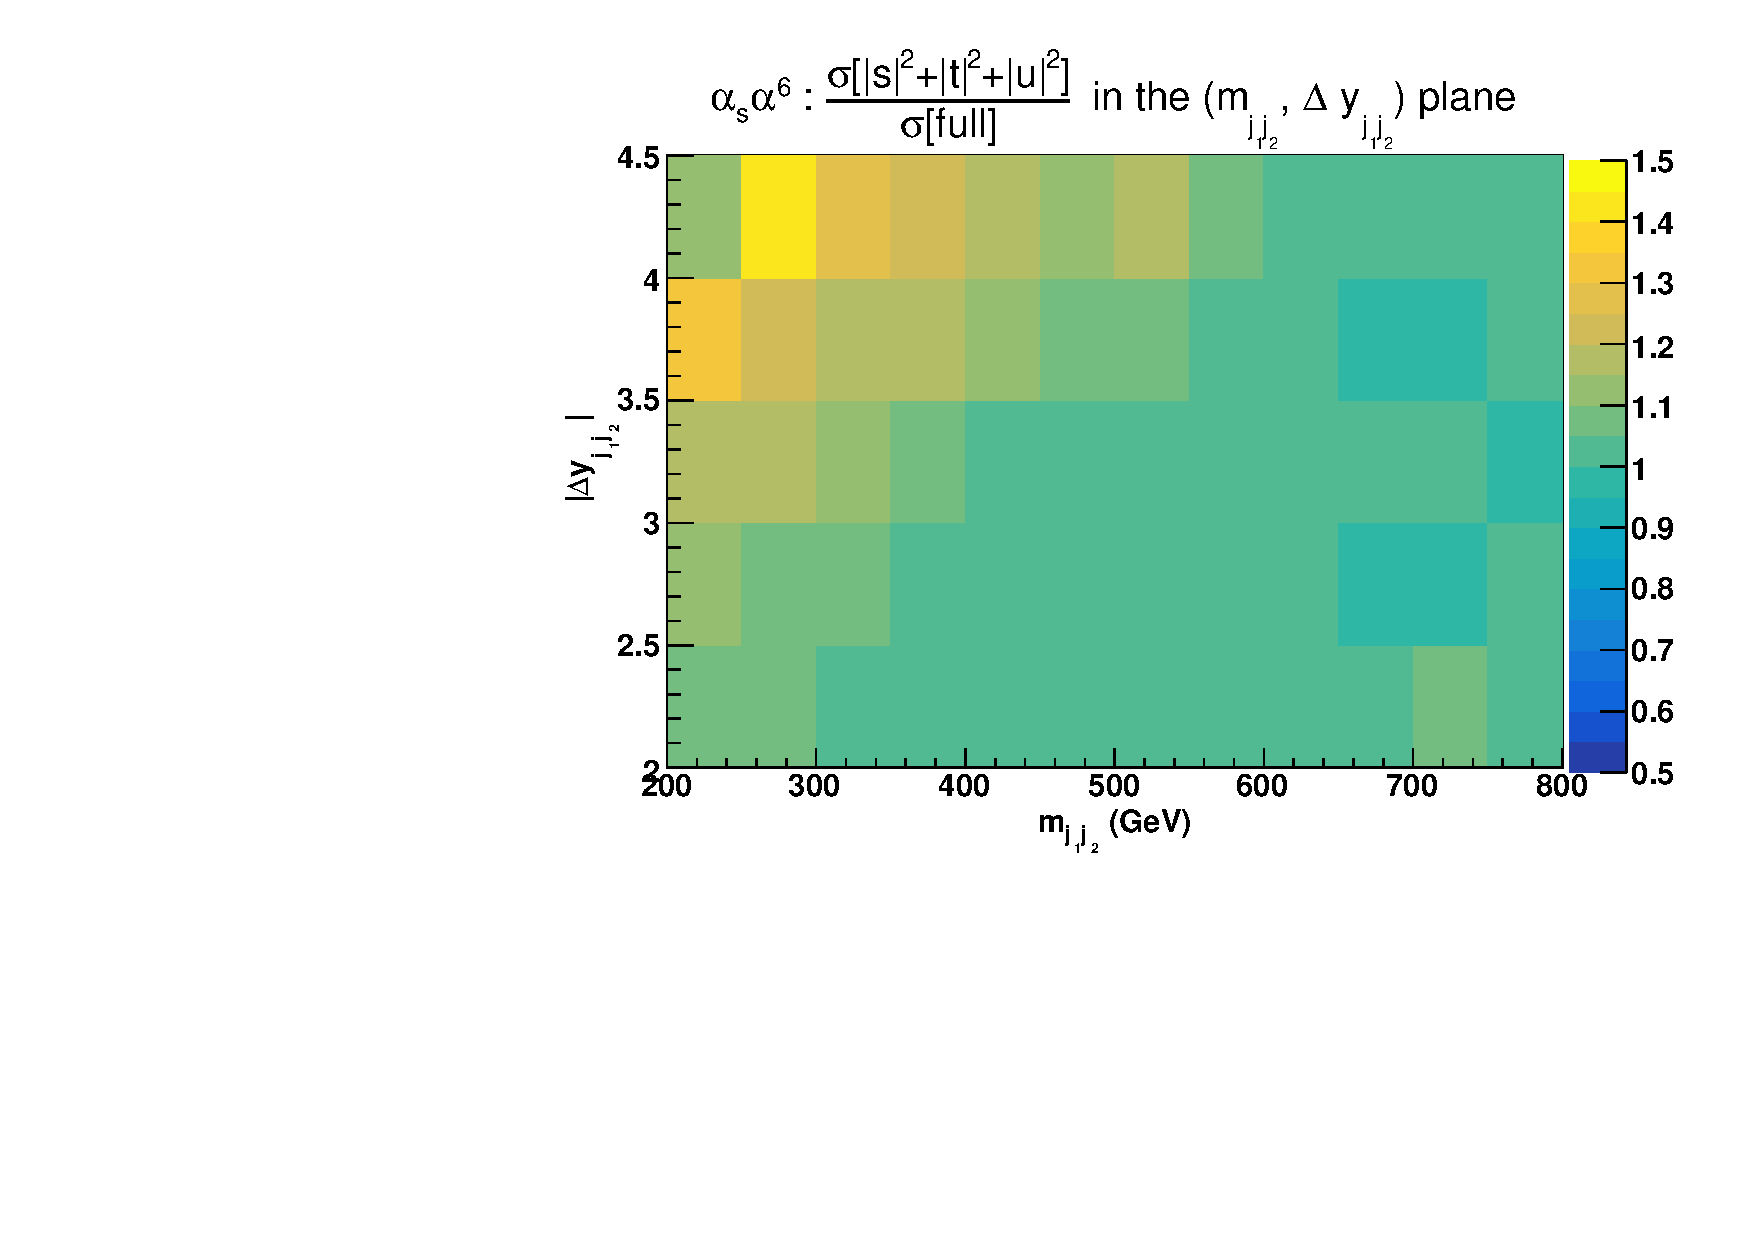
\includegraphics[scale=0.39]{figures/scanfigures/a6as_vbfnloVSrecola_stu.pdf}
FIGURE
\caption{Cross section (fb) per bin of $(M_{jj},\,\Delta y_{jj})$ at NLO QCD $\mathcal{O}(\alpha^6\alphas)$, without any cut on the $jj$ pair kinematics:  ratio of approximated squared amplitudes over the full matrix element. The approximated squared amplitudes are computed as $|\mathcal{A}|^2 \sim |s|^2 + |t|^2 + |u|^2$. Results of \texttt{VBFNLO} (approximated) and \texttt{RECOLA} (full) calculations.}\label{fig:mjjdyjj_2d_NLO}
\end{figure}


\begin{figure}[hbt]
\centering
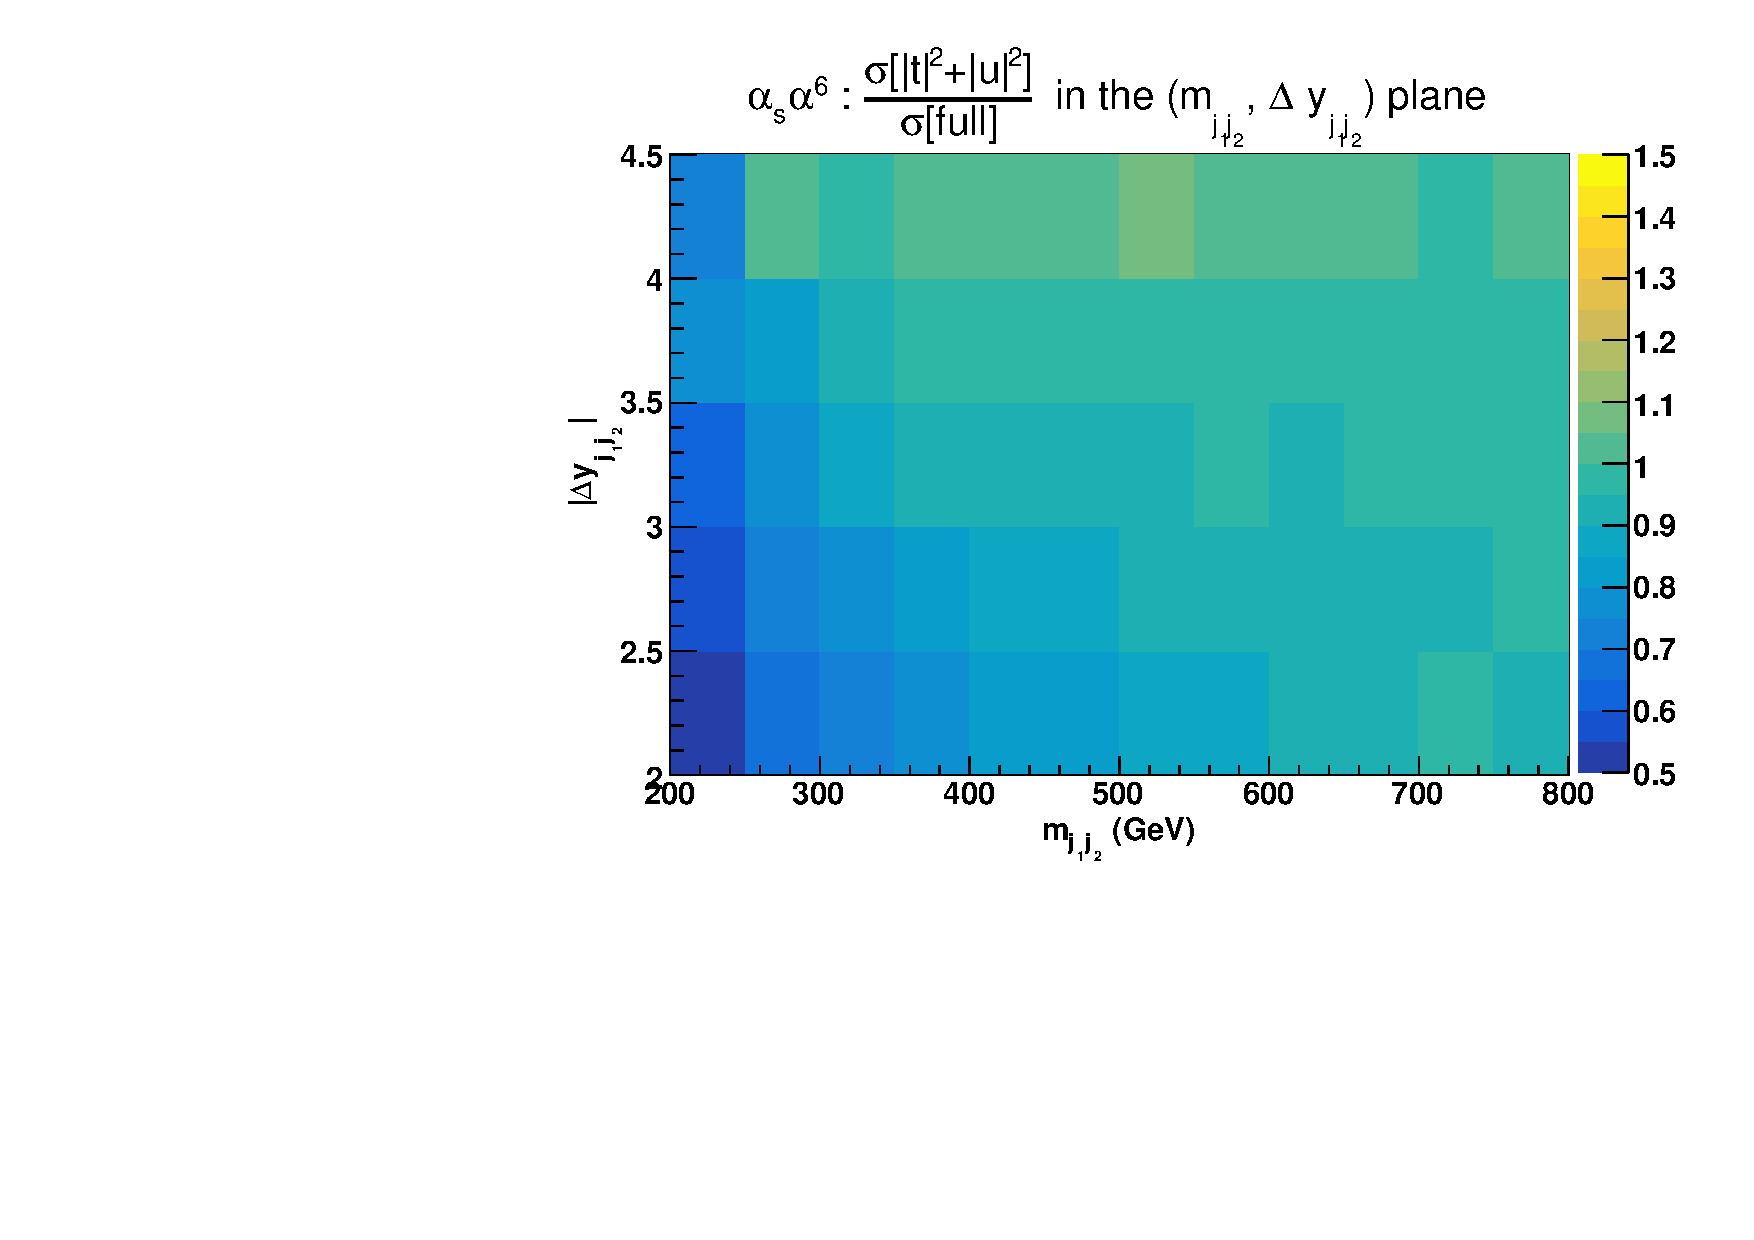
\includegraphics[scale=0.395]{figures/scanfigures/a6as_vbfnloVSrecola_tu.pdf}
%\includegraphics[scale=0.395]{figures/scanfigures/.pdf}
\caption{Cross sections (fb) per bin of $(M_{jj},\,\Delta y_{jj})$ at NLO QCD $\mathcal{O}(\alpha^6\alphas)$, without any cut on the $jj$ pair kinematics: ratio of approximated squared amplitudes over the full matrix element. The approximated squared amplitudes are computed as $|\mathcal{A}|^2 \sim |t|^2 + |u|^2$. Results of \texttt{VBFNLO} (approximated) and \texttt{RECOLA} (full) calculations.}\label{fig:ratio2d_NLO}
\end{figure}